\documentclass[a4paper,11pt]{report}
\usepackage[T1]{fontenc}
\usepackage[utf8]{inputenc}
\usepackage{lmodern,url}
\usepackage{graphicx}
\usepackage{hyperref}
\usepackage{pslatex}
\usepackage{listings}
\usepackage{textcomp}
\usepackage{float}
\usepackage[paper=a4paper,headheight=0pt,left=4cm,top=3cm,right=3cm,bottom=3cm]{geometry}
\usepackage{titling}
\usepackage{pdfpages}
\usepackage{booktabs}
\usepackage[version=4]{mhchem}
\usepackage{isotope}
\usepackage{datetime2}
\usepackage{rotating}
\usepackage{pdflscape}
\usepackage{subfigure}

\DTMsetdatestyle{ddmmyyyy}
\DTMsetup{datesep=--}
\newcommand{\subtitle}[1]{%
  \posttitle{%
    \par\end{center}
    \begin{center}\large#1\end{center}
    \vskip0.5em}%
}
\newcommand{\ra}[1]{\renewcommand{\arraystretch}{#1}}
\newcommand{\addChapter}[1]{\phantomsection \addcontentsline{toc}{chapter}{#1}}
% Tambahkan berkas PDF ke dalam laporan dan gunakan style laporan  
% terhadap berkas ini. 
\newcommand{\inpdf}[1]{
	\includepdf[pages=-,pagecommand={\thispagestyle{fancy}}]{#1.pdf}}
% 
% Tambahkan berkas PDF ke dalam laporan. 
\newcommand{\putpdf}[1]{\includepdf[pages=-]{#1.pdf}}
\renewcommand*\descriptionlabel[1]{\hspace\leftmargin$#1$}
% 
%
% Hyphenation untuk Indonesia 
%
% @author  Andreas Febrian
% @version 1.00
% 
% Tambahkan cara pemenggalan kata-kata yang salah dipenggal secara otomatis 
% oleh LaTeX. Jika kata tersebut dapat dipenggal dengan benar, maka tidak 
% perlu ditambahkan dalam berkas ini. Tanda pemenggalan kata menggunakan 
% tanda '-'; contoh:
% menarik
%   --> pemenggalan: me-na-rik
%

\hyphenation{
    % alphabhet A
    a-na-li-sa a-tur 
    a-pli-ka-si 
    % alphabhet B
    ba-ngun-an 
    be-be-ra-pa 
    ber-ge-rak
    ber-ke-lan-jut-an 
    ber-pe-nga-ruh 
    ber-o-pe-ra-si
    % alphabhet C
    ca-ri cri-ti-cal
    % alphabhet D
    di-sim-pan di-pim-pin de-ngan da-e-rah di-ba-ngun da-pat di-nya-ta-kan 
    di-sim-bol-kan di-pi-lih di-li-hat de-fi-ni-si di-de-fi-ni-si-kan
    di-mo-del-kan di-te-rap-kan
    di-ha-rap-kan
    di-e-va-lu-a-si
    di-su-sun
    di-sa-ji-kan
    % alphabhet E
    e-ner-gi eks-klu-sif
    % alphabhet F
    fa-si-li-tas
    % alphabhet G
    ga-bung-an ge-rak
    % alphabhet H
    ha-lang-an
    % alphabhet I
    % alphabhet J
    % alphabhet K
    ke-hi-lang-an
    ku-ning 
    kua-li-tas ka-me-ra ke-mung-kin-an ke-se-pa-ham-an
    % alphabhet L
    ling-kung-an
    % alphabhet M
    me-ne-ngah
    meng-a-tas-i me-mung-kin-kan me-nge-na-i me-ngi-rim-kan 
    meng-u-bah meng-a-dap-ta-si me-nya-ta-kan mo-di-fi-ka-si
    meng-a-tur
    meng-a-la-mi
    meng-u-kur
    me-re-pre-sen-ta-si-kan
    men-da-pat-kan
    % alphabhet N
    nya-ta non-eks-klu-sif nu-klir
    % alphabhet O
    o-pe-ra-si
    % alphabhet P
	pe-nye-rap-an 
	pe-ngon-trol
    pe-mo-del-an
    pe-ran  pe-ran-an-nya
    pem-ba-ngun-an pre-si-den pe-me-rin-tah prio-ri-tas peng-am-bil-an 
    peng-ga-bung-an pe-nga-was-an pe-ngem-bang-an 
    pe-nga-ruh pa-ra-lel-is-me per-hi-tung-an per-ma-sa-lah-an 
    pen-ca-ri-an peng-struk-tur-an
    per-siap-an pa-ra-me-ter
    pa-sang-an
    % alphabhet Q
    % alphabhet R
    ran-cang-an
    % alphabhet S
    si-mu-la-si sa-ngat
    se-dang-kan sa-tu-an
    % alphabhet T
    te-ngah
    ter-da-pat
    % alphabhet U
    % alphabhet V
    % alphabhet W
    % alphabhet X
    % alphabhet Y
    % alphabhet Z
    % special
}

\definecolor{amber}{rgb}{0.96, 0.51, 0.13}
\definecolor{biruMuda}{rgb}{0.45, 0.62, 0.78}

\renewcommand{\contentsname}{Daftar Isi}
\renewcommand{\chaptername}{BAB}
\renewcommand{\bibname}{Daftar Referensi}
\renewcommand{\listfigurename}{Daftar Gambar}
\renewcommand\lstlistlistingname{Daftar Program}
\renewcommand{\figurename}{Gambar}
\renewcommand{\tablename}{Tabel}
%\title{Lampiran II}
%\title{Kajian Komputasi Dinamika Fluida berbasis OpenFOAM}
%\author{Arya Adhyaksa Waskita}
%\date{January 31, 2017}
\begin{document}
\begin{titlepage}

\newcommand{\HRule}{\rule{\linewidth}{0.5mm}} % Defines a new command for the horizontal lines, change thickness here

\center % Center everything on the page


%----------------------------------------------------------------------------------------
%	LOGO SECTION
%----------------------------------------------------------------------------------------


\includegraphics[scale=.25]{pics/logo.png}\\[1cm] % Include a department/university logo - this will require the graphicx package

%----------------------------------------------------------------------------------------
%	TITLE SECTION
%----------------------------------------------------------------------------------------

\HRule \\[0.4cm]
{ \huge \bfseries Dokumen Pengembangan TRIAC2 \\ (TRIso \textit{Analysis Code coupled with Fresco capabilities})}\\[0.4cm] % Title of your document
\HRule \\[1.5cm]

%----------------------------------------------------------------------------------------
%	HEADING SECTIONS
%----------------------------------------------------------------------------------------
%\textsc{Sub Bidang Termohidrolika}\\[0.25cm] % Minor heading such as course title
\textsc{Laboratorium Komputasi}\\[0.25cm] % Major heading such as course name
\textsc{\Large Pusat Teknologi dan Keselamatan Reaktor Nuklir}\\[1.5cm] % Name of your university/college

 
%----------------------------------------------------------------------------------------
%	AUTHOR SECTION
%----------------------------------------------------------------------------------------

\begin{minipage}{0.4\textwidth}
\begin{flushleft} \large
\emph{Disusun oleh:}\\
Arya Adhyaksa Waskita
\end{flushleft}
\end{minipage}
~
\begin{minipage}{0.4\textwidth}
\begin{flushright} \large
\emph{Supervisor:} \\
Dr. Eng. Topan Setiadipura
\end{flushright}
\end{minipage}\\[4cm]

% If you don't want a supervisor, uncomment the two lines below and remove the section above
%\Large \emph{Author:}\\
%John \textsc{Smith}\\[3cm] % Your name

%----------------------------------------------------------------------------------------
%	DATE SECTION
%----------------------------------------------------------------------------------------

{\large 30/09/2019}\\[3cm] % Date, change the \today to a set date if you want to be precise
%{\large 31 Juli 2017}\\[3cm] % Date, change the \today to a set date if you want to be precise
 
%----------------------------------------------------------------------------------------

\vfill % Fill the rest of the page with whitespace

\end{titlepage}

%\tableofcontents

\pagenumbering{roman}
%\maketitle
\clearpage
\setcounter{page}{2}
\addChapter{Daftar Gambar}
\tableofcontents
%\clearpage
\listoffigures
\addChapter{Daftar Program}
\lstlistoflistings
%\clearpage
\pagenumbering{arabic}

\chapter{Pendahuluan}
\section{Latar Belakang}
Analisis keselamatan reaktor nuklir melibatkan sejumlah aspek seperti diperlihatkan pada \figurename~\ref{fig:aspek}. Setelah upaya melakukan rekayasa balik terhadap PANAMA \cite{report1,VERFONDERN201484} untuk aspek kinerja bahan bakar \cite{triac1}, dipandang perlu untuk melanjutkan analisis keselamatan di aspek \textit{radiactive release}.

\begin{figure}[h!]
  \begin{center}
    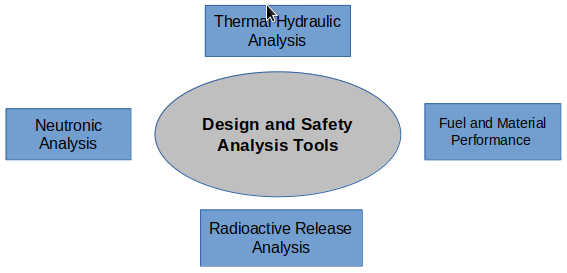
\includegraphics[scale=.5]{pics/tools.png}
    \caption{Aspek keselamatan reaktor nuklir}
    \label{fig:aspek}
  \end{center}
\end{figure}

Kode komputer FRESCO \cite{report2} sebagai salah satu kode baku dalam analisis keselamatan reaktor di pelepasan radionuklida yang turut menghantarkan Jerman sebagai \textit{center of excellent} pada penelitian tersebut. 

\chapter{Dasar Teori}

\section{Lepasan Radionuklida}
Fenomena pelepasan radionuklida yang dimodelkan oleh FRESCO adalah lepasnya produk fisi dari sebuah bahan bakar \textit{pebble bed}. Fenomena tersebut dapat diilustrasikan pada \figurename~\ref{fig:produkFisiLepas}. Lingkaran kuning yang terlihat di \figurename~\ref{fig:produkFisiLepas} adalah partikel TRISO yang telah dikembangkan sebelumnya dalam TRIAC \cite{triac1}. Sedangkan lingkaran besar yang melingkupi partikel TRISO adalah bahan bakar \textit{pebble bed}.

\begin{figure}[h!]
  \begin{center}
    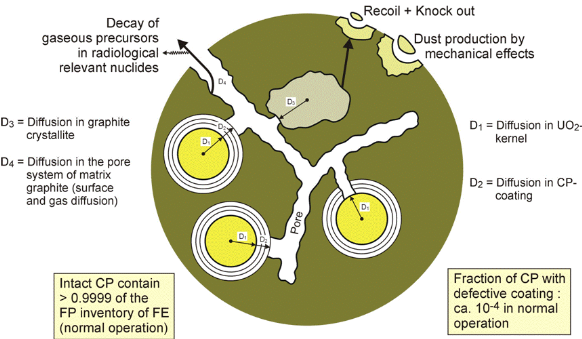
\includegraphics[scale=.5]{pics/ilustrasiLepas.png}
    \caption{Ilustrasi lepasnya produk fisi dari bahan bakar \textit{pebble bed} \cite{report2}}
    \label{fig:produkFisiLepas}
  \end{center}
\end{figure}

Hasil analisis yang diharapkan adalah lepasnya radionuklida tersebut dari gedung reaktor yang diagram skematiknya diilustrasikan pada \figurename~\ref{fig:reaktorHTRskematik}. Jika peluang terlepasnya radionuklida tersebut rendah, maka semakin rendah pula peluang terlepasnya radionuklida tersebut ke lingkungan. Hal ini dipengaruhi sejumlah penghalang yang ada di reaktor sebelum radionuklida tersebut terlepas ke lingkungan. Dan jika memang dapat terlepas sampai ke lingkungan, maka radionuklida tersebut telah mengalami peluruhan aktivitas dengan tingkat yang berbeda, tergantung jenis radionuklidanya \cite{report3}.

\begin{figure}[h!]
  \begin{center}
    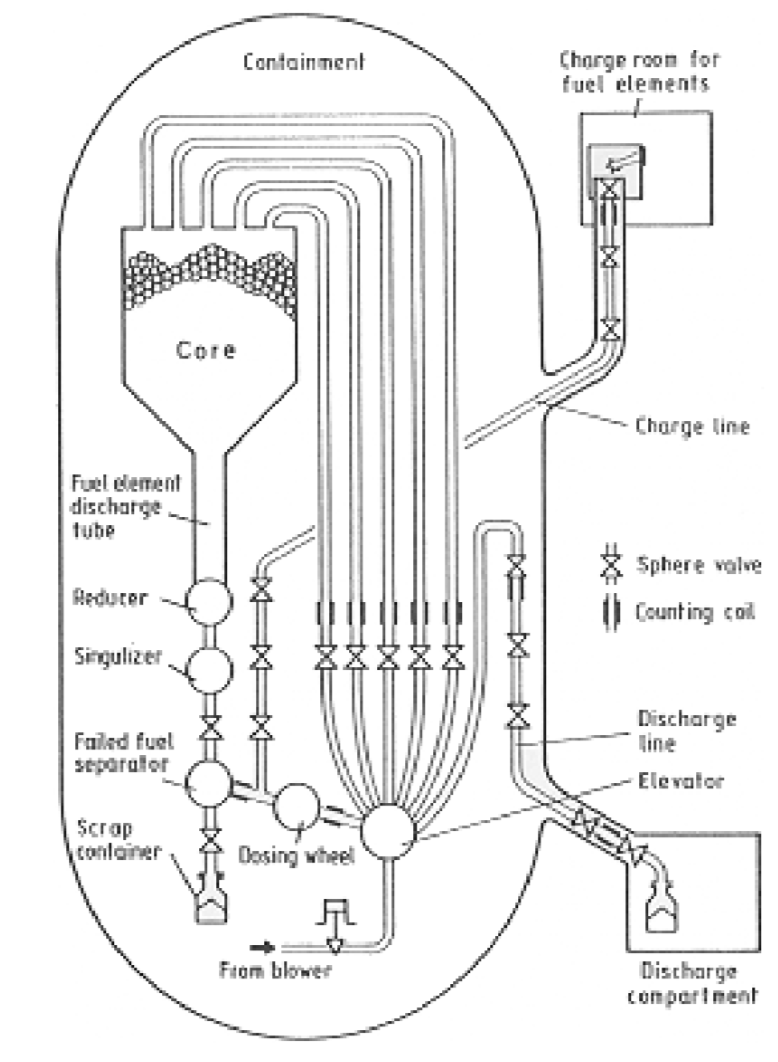
\includegraphics[scale=.25]{pics/htrSchematic.png}
    \caption{Diagram skematik reaktor temperatur tinggi \cite{kadak}}
    \label{fig:reaktorHTRskematik}
  \end{center}
\end{figure}

Jumlah radionuklida produk fisi dapat ditentukan menggunakan persamaan \ref{eq:jmlProdukFisi} \cite{report2}
\begin{equation}
\frac{dN}{dt}=\sum\limits_{i=1}^{n}Y_if_i - \lambda N
\label{eq:jmlProdukFisi}
\end{equation}

Dengan waktu paruh dari setiap isotop dinyatakan sebagai persamaan \ref{eq:wktParuh}
\begin{equation}
  T_{\frac{1}{2}}=\frac{\ln 2}{\lambda}
  \label{eq:wktParuh}
\end{equation}

Dengan mengabaikan faktor prekursor serta penyerapan netron yang terjadi, ketika nilai fisi yang terjadi mendekati konstan, maka aktifitas produk fisi dapat dinyatakan sebagai persamaan \ref{eq:activity} \cite{report3}
\begin{equation}
  A=\lambda N = \sum\limits_{i=1}^{n}Y_if_i\left(1-\exp^{-\lambda t} \right)
  \label{eq:activity}
\end{equation}

Pada produk fisi yang memiliki waktu paruh pendek, kesetimbangan aktifitas dapat diperoleh secara cepat dan dapat diformulasikan sebagai persamamaan \ref{eq:waktuparuhpendek} \cite{report2}.
\begin{equation}
  A=\sum\limits_{i=1}^nY_if_i
  \label{eq:waktuparuhpendek}
\end{equation}

Berikut adalah definisi dari simbol yang ada di persamaan \ref{eq:jmlProdukFisi} - \ref{eq:waktuparuhpendek}.
\begin{itemize}
  \item $N$: jumlah atom produk fisi ($\frac{atom}{barn.cm}$)
  \item $Y-i$: hasil fisi
  \item $F_i$: laju fisi ($s^{-1}$)
  \item $n$: jumlah isotop waktu ke-$n$
  \item $\lambda$: konstanta peluruhan ($s^{-1}$)
  \item $A$: aktifitas produk fisi ($Bq$)
  \item $t$: waktu ($s$)
\end{itemize}

Dalam kondisi operasi (normal atau tidak), energi kinetik dalam reaktor berada pada keadaan tinggi. Produk fisi yang lahir akan bergerak pada jarak tertentu antara \textit{buffer} dan pelapis kernel. Hal ini menyebabkan beberapa produk fisi yang terbentuk di permukaan kernel akan bergerak dan berkumpul di daerah \textit{buffer}. Fenomena ini dikenal sebagai \textit{recoil effect} yang dapat dihitung dengan persamaan \ref{eq:reqoil} \cite{report3}.
\begin{equation}
  F_{recoil}=\frac{\int_{r_0-R}^{R}\frac{2Rr-\left(r_0^2-R^2\right)+r^2}{4Rr}}{\frac{4\pi r_0^3}{3}}
  \label{eq:reqoil}
\end{equation} 

Persamaan \ref{eq:reqoil} dapat dituliskan sebagai persamaan \ref{eq:reqoil2} \cite{report3}
\begin{equation}
  F_{recoil}=\frac{3}{4}\frac{r}{r_0}\left[1-\frac{1}{12}\left(\frac{R}{r_0}\right)^2\right]
  \label{eq:reqoil2}
\end{equation}

Sedangkan simbol pada persamaan \ref{eq:reqoil} dan \ref{eq:reqoil2} adalah sebagai berikut.
\begin{itemize}
  \item $F_{recoil}$: fraksi isotop ke daerah \textit{buffer} ($\frac{matrix}{grain}$)
  \item $r_0$: radius kernel ($m$)
  \item $R$: jarak \textit{recoil} ($m$)
\end{itemize}

Pada bagian batas antara bahan bakar dan \textit{coolant}, terdapat transisi yang terjadi pada atom yang diakibatkan oleh proses adsorpsi dan desorpsi (evaporasi). Kedua proses ini berbeda satu dengan yang lainnya dan dinamakan sebagai efek sorpsi. Sebaran konsentrasi isotop pada proses adsorpsi dan desorpsi diilustrasikan pada \figurename~\ref{fig:efeksorpsi}.

\begin{figure}
  \begin{center}
    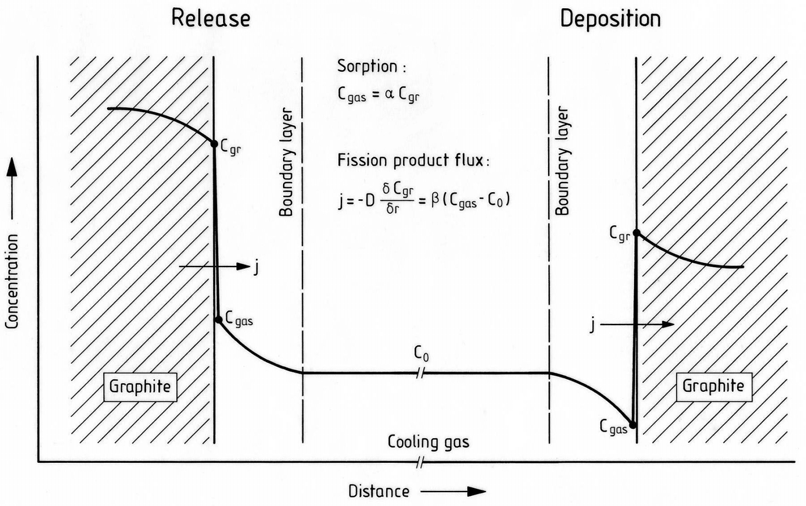
\includegraphics[scale=.35]{pics/efeksorpsi.png}
    \caption{Persebaran konsentraasi isotop tinjauan pada proses adsorpsi dan desorpsi \cite{report2}}
    \label{fig:efeksorpsi}
  \end{center}
\end{figure}

Efek sorpsi sangat tergantung pada nuklida yang ditinjau pada \textit{bulk} dan \textit{coolant}, kondisi termodinamika yang dialami, dan tipe dari grafit yang digunakan. Selain itu, kecepatan \textit{coolant} (\textit{mass flow rate}) memiliki dampak pada efek sorpsi. Pada komponen bahan bakar, terdapat komponen yang dinamakan sebagai \textit{coked phenolic resin binder}. Komponen tersebut memiliki karakterisitik nilai kapasitas sorpsi yang tinggi untuk Cs (cesium) dan Sr (stronsium), tetapi rendah untuk Ag (silver) dan I (iod). Sedangkan kapasitas sorpsi dari I berbanding terbalik dengan nilai temperatur \cite{report3}.

\section{FRESCO II}
Dalam FRESCO-II terdapat 35 subrutin yang dapat dikelompokan menjadi tiga, yang masing-masing adalah data masukan, perhitungan fisis dan solusi. Yang dimaksud dengan perhitungan fisis adalah perhitungan berdasarkan sifat fisis dari fenomena yang terjadi. Sedangkan subrutin solusi adalah subrutin yang digunakan untuk menyelesaikan persamaan linier dalam bentuk matriks dan interpolasi data \cite{report3}.

Prosedur kalkulasi didalam tiap waktu tinjauan dilakukan dengan dua bagian, yaitu kalkulasi \textit{diffusive release} dari partikel \textit{intact} dan \textit{devective} dari \textit{graphite grain} yang terkonduksi. Jumlah dari semua keluaran produk fisi akan dihitung sebagai total sumber yang akan berpengaruh terhadap kalkulasi matriks \textit{graphite} \cite{report2}, Bagian yang kedua akan mengkalkulasi \textit{diffusive transport} pada bagian batas \textit{graphite grain} melalui matriks dan lepasan oleh desorpsi dari permukaan \textit{fuel sphere} (\textit{microsphere}) ke arah \textit{coolant}.

Terdapat beberapa asumsi yang digunakan oleh FRESCO II. Salah satu kalkulasi sederhana yang digunakan adalah setiap radionuklida yang akan dihitung diasumsikan sama seperti produk fisi yang berarti tinjauannya hanya pada pada waktu paruhnya saja pada fluks konstan \cite{report3}.

Perhitungan model difusi yang digunakan didasarkan pada solusi numerik dari hukum Fick untuk tinjauan \textit{transport} produk fisi yang terjadi pada kernel, layer pelapis, dan grafit matriks dari elemen bahan bakar sebagai fungsi yang bergantung pada temperature tiap waktu \cite{report2}. Solusi numerik diperoleh dari persamaan diferensial difusi pada koordinat bola. Bola tinjauan akan dibagi oleh N kulit bola yang berarti terdapat N bagian volume bernilai Vi dengan nilai koefisien difusi yang dinyatakan sebagai Di, dimana i = 1, . . . ,N., dan sumber fisi konstan Q, skema dapat dilihat pada \figurename~\ref{fig:diskritisasi}. Konsentrasi pada tiap bagian dianggap sama terkecuali pada posisi tengah atau i = N. 

\begin{figure}[h!]
  \begin{center}
    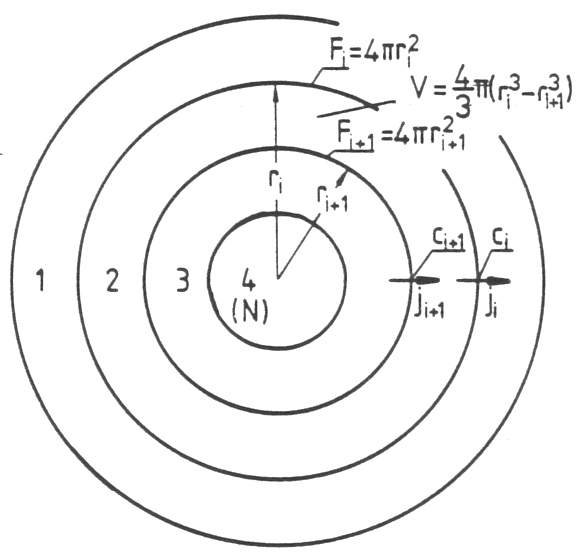
\includegraphics[scale=.35]{pics/diskritisasiFuel.png}
    \caption{Diskritisasi elemen bahan bakar}
    \label{fig:diskritisasi}
  \end{center}
\end{figure}

Pada bagian tegah yang memiliki sumber, berlaku persamaan konsentrasi yang didapat secara kuadratik mengikuti persamaan \ref{eq:kuadratik}. 
\begin{equation}
  C=C_N-2\frac{C_{N+1}-C_N}{r_N}\left(r-r_N\right)-\frac{C_{N+1}-C_N}{r_N^2}\left(r-r_N\right)^2
  \label{eq:kuadratik}
\end{equation}

Kemudian, laju massa produk fisinya mengikuti persamaan \ref{eq:lajumassa}.
\begin{equation}
  j=-2D_N\frac{C_{N+1}-C_N}{-r_N}
  \label{eq:lajumassa}
\end{equation}

Untuk bagian lain (selain bagian tengah) di mana $i \neq N$, berlaku persamaan \ref{eq:bukanditengah} dan laju massa produk fisinya mengikuti persamaan \ref{eq:lajumassadii}. 
\begin{equation}
  C=C_i+\frac{C_{i+1}-C_i}{r_{i+1}-r_i}\left(r-r_i\right)
  \label{eq:bukanditengah}
\end{equation}

\begin{equation}
j=-D_i\frac{C_{i+1}-C_i}{r_{i+1}-r_i}
\label{eq:lajumassadii}  
\end{equation}

Setelah dilakukan kalkulasi produk fisi dengan tinjauan diskrit pada daerah yang ditentukan, penentuan massa rata-rata produk fisi pada elemen volume $V_i$  dinyatakan sebagai persamaan \ref{eq:Vi}.
\begin{equation}
  \frac{d}{dt}\int_{v_i}c dV = QV_i-\lambda \int_{v_i}-j_iF_i + j_{i+1}F_{i+1}
  \label{eq:Vi}
\end{equation}

Sedangkan simbol-simbil yang digunakan pada persamaan \ref{eq:kuadratik}-\ref{eq:Vi} memiliki makna berikut.
\begin{itemize}
  \item $c$: konsentrasi ($\frac{mMol}{kg}$)
  \item $r$: jari-jari tinjauan ($m$)
  \item $r_i$: jari-jari kulit ke-$i$
  \item $j$: laju massa produk fisi ($\frac{mMol}{s.kg}$)
  \item $D_i$: konstanta difusi pada kulit ke-i ($\frac{m^2}{s}$)
  \item $F$: fraksi lepasan
  \item $t$: waktu(s)
\end{itemize}

Dengan mengasumsikan bahwa konsentrasi dari produk fisi yang dihasilkan hanya bergantung pada arah radial, maka persamaan umumnya dapat dinyatakan sebagai persamaan \ref{eq:arahradial}. 
\begin{equation}
  \frac{\partial c}{\partial t}=\frac{1}{r^2}\frac{\partial}{\partial r} \left[r^2\left[D(r)\frac{\partial c}{\partial r}\right] \right]+w(r)-\lambda c
  \label{eq:arahradial}
\end{equation}

Jika dilakukan pembagian daerah seperti yang digambarkan pada \figurename~\ref{fig:diskarahradial}, persamaan \ref{eq:arahradial} akan menjadi persamaan \ref{eq:arahradial2} \cite{keshaw}.

\begin{figure}[h!]
  \begin{center}
    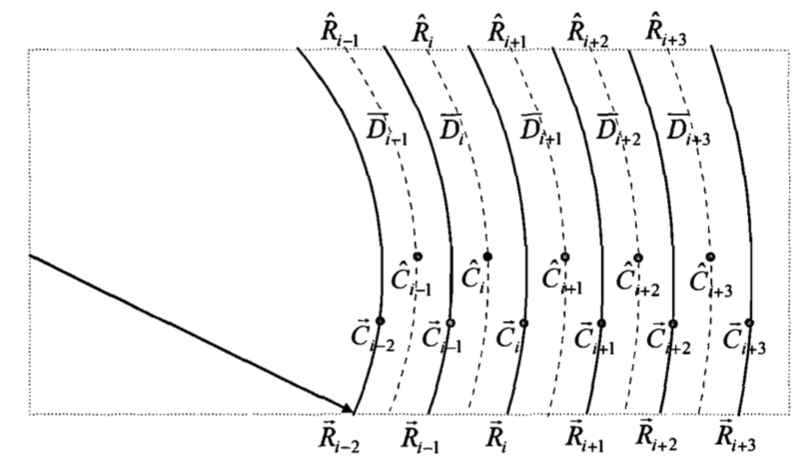
\includegraphics[scale=.35]{pics/arahradial.png}
    \caption{Diskritisasi arah radial \cite{keshaw}}
    \label{fig:diskarahradial}
  \end{center}
\end{figure}

\begin{equation}
\frac{\partial \hat{c_i}}{\partial t}=\frac{1}{\hat{R_i^2}}\frac{\left[\vec{R}_i^2\left[D_i\left|\frac{\partial c}{\partial r}\right|\right] -\vec{R}_{i-1}^2\left[D_{i-1}\left|\frac{\partial c}{\partial r}\right|\right]\right]}{\vec{R}_i-\vec{R}_{i-1}}
\label{eq:arahradial2}
\end{equation}

dengan:
\begin{itemize}
  \item $\hat{c}$: konsentrasi pada daerah tengah elemen partisi ($\frac{mMol}{kg}$)
  \item $\hat{R}$: jari-jari $\hat{c}$  tinjauan $m$
  \item $r_i$: jari-jari kulit ke-$i$ ($m$)
  \item $\vec{R}$: jari-jari tinjauan elemen ke-$i$ ($m$)
  \item $D_i$: konstanta difusi pada kulit ke-$i$ ($\frac{m^2}{s}$)
  \item $w_i$: rata-rata densitas produks fisi pada daerah partisi ke-$i$
\end{itemize}

Dari persamaan \ref{eq:arahradial2} dapat dibentuk matriks yang berbentuk matriks tridiagonal dan penyelesaiannya dapat dilakukan menggunakan metode gauss atau metode LU.

\chapter{Struktur Program}
\section{Diagram konteks}
Sistem yang akan dikembangkan memiliki diagram konteks level 0 seperti pada \figurename~\ref{fig:level0}. Triac2 akan menerima masukan berupa fraksi gagal bahan bakar dan menghasilkan fraksi lepasan radionuklida. 

\begin{figure}[h!]
  \begin{center}
    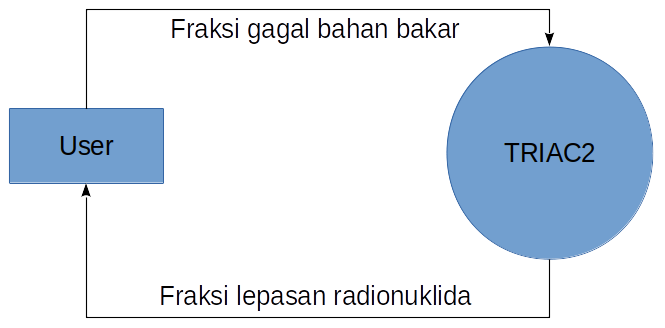
\includegraphics[scale=.5]{pics/contextLevel0.png}
    \caption{Konteks level 0 dari sistem TRIAC2}
    \label{fig:level0}
  \end{center}
\end{figure}

\section{Kebutuhan fungsi}
Seperti yang telah dijelaskan FRESCO II menggunakan 3 jenis sub rutin, yang masing-masing bertujuan untuk mengelola berkas masukan, melakukan perhitungan fenomena fisi serta penyelesaian persamaan matriks. Berkas masukan FRESCO II sendiri berikut penjelasannya dapat diilustrasikan pada \figurename~\ref{fig:fileinput}. Sehingga kebutuhan pertama yang harus dimiliki TRIAC2 adalah kemampuan untuk membaca data tersebut untuk selanjutnya dihitung.

\begin{figure}[h!]
  \begin{center}
    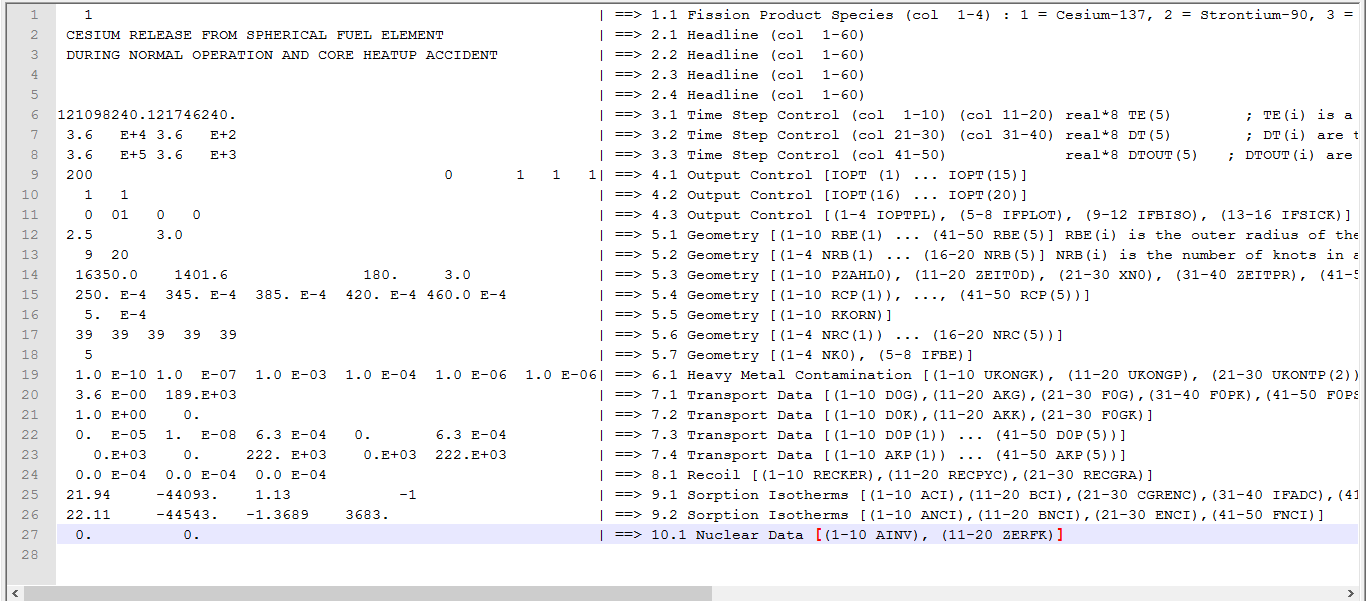
\includegraphics[scale=.25]{pics/inputFresco.png}
    \caption{Berkas masukan dan penjelasannya}
    \label{fig:fileinput}
  \end{center}
\end{figure}

Selanjutnya, FRESCO II akan menghasilkan sejumlah nilai berikut. Fungsi-fungsi tersebut akan dijalankan oleh subrutin yang bertugas melakukan kalkulasi fenomena fisi
\begin{enumerate}
  \item Fraksi lepasan dan rerata fraksi gagal untuk seluruh partikel \textit{pebbel bed}
  \item Inventarisasi produk fisi pada seluruh partikel
  \item Inventarisasi produk fisi pada \textit{coated particle} (partikel triso)
  \item Jumlah produk fisi yang lepas
  \item Laju lepasan ($\frac{1}{s}$)
\end{enumerate}

Dalam FRESCO II, kalkulasi fenomena fisis diterapkan dalam sejumlah subrutin yang dijelaskan pada \tablename~\ref{tab:daftarsubrutin}.

\begin{table}[h!]
  \caption{Daftar fungsi dan subrutin pada FRESCO-II}
  \label{tab:daftarsubrutin}
  \begin{center}
    \begin{tabular}{p{3cm}p{10cm}} \toprule
    Fungsi / Subrutin & Deskripsi\\ \midrule
    ANFANG & Tetapkan profil konsentrasi pada awal kecelakaan \\ \hline
    BEDIFF (FREICP, CGM) & Perhitungan transportasi produk fisi dalam grafit\\ \hline
    BRUCHP (PZAHL0, IFJN) & Lepasan dari partisi partikel yang rusak\\ \hline
    INSTAT & Perhitungan pelepasan produk fisi keadaan \textit{unsteady}\\ \hline
    KUDIF (N, R, DTI, UEZ, DI, Q, ZERFK, T0, T, GES) & Integrasi numerik difusi produk fisi untuk bahan bakar bola untuk satu langkah waktu\\ \hline
    PADIFF (FREI, C00) & Perhitungan difusi produk fisi dari partikel dan dari butiran grafit (recoil diperhitungkan dalam fungsi sumber)\\ \hline
    RADIF (R, N, R2, N1, N2) & Partisi bola dalam zona untuk perhitungan difusi\\ \hline
    RECOIL (Q, RCFRPK, RCFRP) & Perhitungan pelepasan recoil dari kernel, partikel, dan elemen bahan bakar.\\ \hline
    SICOR (TT) & Perhitungan penipisan lapisan SiC karena korosi\\ \hline
    ZOZA (R, N) & Penentuan jumlah zona dengan data transportasi berbeda\\ \hline
    ADSORP (T,C) & Perhitungan rasio antara konsentrasi lapisan batas dan konsentrasi permukaan dari isoterm sorpsi untuk grafit A3 Matriks\\ \hline
    AINVE (R, C, N1, N2) & Integrasi konsentrasi dalam cangkang bola antara posisi $N_1$ dan $N_2$ (profil linier di antaranya)\\ \hline
    BETA (V, P, T) & Koefisien perpindahan massa pada grafit batas / helium\\ \hline
    DIFKO(T) & Koefisien difusi untuk butiran grafit\\ \hline
    DIFPA (T, I) & Koefisien difusi. Untuk kernel dan lapisan partikel. I: jumlah zona partikel, 1 = pusat.\\ \hline
    DIFPAD (T,I) & Koefisien difusi. untuk kernel partikel cacat CP. I: jumlah zona partikel, 1 = pusat.\\ \hline
    DIFPO (T,I) & Koefisien difusi. Dalam pori-pori grafit, I: jumlah zona grafit, 1 = tengah.\\ \hline
    PBRUCH (ZEIT,TEMPER) & Fungsi kegagalan partikel\\ \hline
    QUELLK (ZEIT) & Fungsi bergantung waktu dan lokasi untuk sumber produk fisi dalam butir grafit\\ \hline
    QUELLP (I) & Fungsi bergantung waktu dan lokasi untuk sumber produk fisi dalam partikel\\ \hline
    QUPOR (ZEIT) & Fungsi bergantung waktu dan lokasi untuk sumber produk fisi dalam pori-pori grafit.\\ \hline
    TEMP (ZEIT) & Suhu elemen bahan bakar \\ 
      \bottomrule
    \end{tabular}
  \end{center}
\end{table}

Kebutuhan fungsi yang ketiga adalah penyelesaian persamaan matriks, dalam hal ini adalah metode eliminasi gauss. Penyelesaian persamaan matriks akan menjadi bagian dari fungsi kalkulasi fenomena fisis. Dalam FRESCO-II, kebutuhan tersebut diterapkan melalui subrutin berikut, seperti dijelaskan dalam \tablename~\ref{tab:daftarsubrutin2}.

\begin{table}[h!]
  \caption{Daftar fungsi dan subrutin pada FRESCO-II}
  \label{tab:daftarsubrutin2}
  \begin{center}
    \begin{tabular}{p{3cm}p{10cm}} \toprule
    Fungsi / Subrutin & Deskripsi\\ \midrule
    TRIDAG (N, A, B, C, D, T) & Solusi sistem persamaan tridiagonal menggunakan prosedur eliminasi gauss\\ \hline
    POLAT (X, X1, X2, Y1, Y2) & Interpolasi linier \\
      \bottomrule
    \end{tabular}
  \end{center}
\end{table}

Hubungan saling keterkaitan antar subrutin yang dijelaskan pada \tablename~\ref{tab:daftarsubrutin} dan \ref{tab:daftarsubrutin2} dijelaskan pada sejumlah gambar berikut. \figurename~\ref{fig:interaction0} mengilustrasikan subrutin yang langsung berada di bawah FRESCO-II.

\begin{figure}[h!]
  \begin{center}
    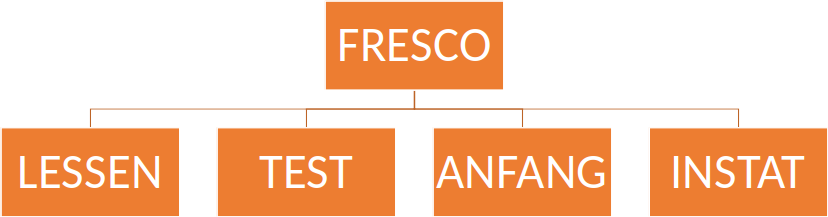
\includegraphics[scale=.35]{pics/intertaction0.png}
    \caption{Subrutin yang langsung berada di bawah FRESCO-II}
    \label{fig:interaction0}
  \end{center}
\end{figure}

Selanjutnya, subrutin LESSEN akan berhubungan dengan subrutin lainnya seperti dijelaskan pada \figurename~\ref{fig:interaction1}.
\begin{figure}[h!]
  \begin{center}
    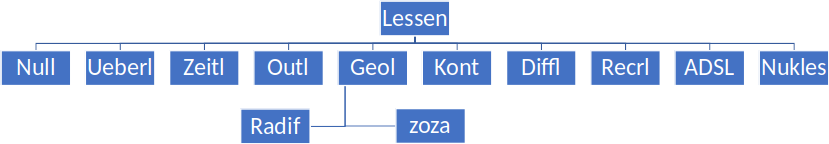
\includegraphics[scale=.35]{pics/intertaction1.png}
    \caption{Interaksi antara subrutin LESSEN dan subrutin lain}
    \label{fig:interaction1}
  \end{center}
\end{figure}

Subrutin ANFANG berinteraksi dengan subrutin berikut seperti dijelaskan pada \figurename~\ref{fig:interaction2}.
\begin{figure}[h!]
  \begin{center}
    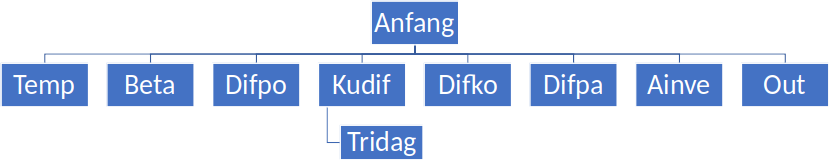
\includegraphics[scale=.35]{pics/intertaction2.png}
    \caption{Interaksi antara subrutin ANFANG dan subrutin lain}
    \label{fig:interaction2}
  \end{center}
\end{figure}

Sedangkan interaksi antara subrutin INSTAT dan subrutin pendukung lainnya dijelaskan pada \figurename~\ref{fig:interaction3}
\begin{figure}[h!]
  \begin{center}
    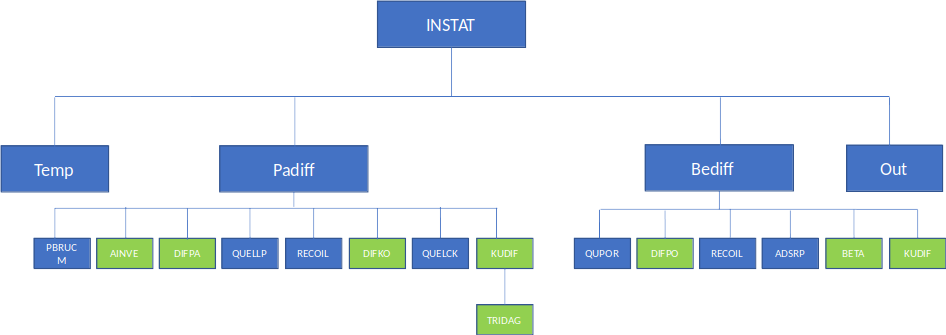
\includegraphics[scale=.4]{pics/intertaction3.png}
    \caption{Interaksi antara subrutin INSTAT dan subrutin lain}
    \label{fig:interaction3}
  \end{center}
\end{figure}
% Daftar Pustaka
\bibliographystyle{IEEEtran}
\bibliography{references}

%\begin{appendix}
%	\include{markLampiran}
%	\setcounter{page}{2}
%	%-----------------------------------------------------------------------------%
\addChapter{Lampiran 1}
\chapter*{Lampiran 1: Contoh file input}
\label{lamp:inputExample}
%-----------------------------------------------------------------------------%
\includepdf[pages={1-}]{THERMIXInputManual.pdf}
%\includepdf{inputExample2}


%\putpdf{THERMIXInputManual}
%\end{appendix}

\end{document}
